\documentclass[10pt,aspectratio=169]{beamer}
%\documentclass[10pt]{beamer}

\usetheme[sectionpage=none] % TODO solve the arithmetic error problem later (on section pages)
  {metropolis}
\usepackage{appendixnumberbeamer}

\usepackage{verbatim}

% strikethrough
% - normalem: do not redefine emph to do underline
\usepackage[normalem]{ulem}

% bold math
\usepackage{bm}

\usepackage{xcolor,soul}
\definecolor{lightblue}{rgb}{.90,.95,1}
\definecolor{lightred}{rgb}{1,.80,.80}
\definecolor{lightgreen}{rgb}{.80,1.,.80}
%\definecolor{lightred}{red!40}
\sethlcolor{lightblue}

\definecolor{rosenpass-pink}{RGB}{247, 4, 132}
\definecolor{rosenpass-orange}{RGB}{255, 166, 48}
\definecolor{rosenpass-gray}{RGB}{64, 63, 76}
\definecolor{rosenpass-lightblue}{RGB}{211, 243, 238}
\definecolor{rosenpass-blue}{RGB}{114, 161, 229}

\setbeamercolor{progress bar}{fg=rosenpass-pink,bg=blue}
\setbeamercolor{title separator}{fg=rosenpass-pink,bg=blue}


\renewcommand<>{\hl}[1]{\only#2{\beameroriginal{\hl}}{#1}}
\usepackage[beamer]{hf-tikz}
% https://tex.stackexchange.com/questions/41683/why-is-it-that-coloring-in-soul-in-beamer-is-not-visible
\makeatletter
\newcommand\SoulColor{%
  \let\set@color\beamerorig@set@color
  \let\reset@color\beamerorig@reset@color}
  \makeatother
  \SoulColor

\setlength{\fboxsep}{0pt}
\newcommand{\mathcolorbox}[2]{\colorbox{#1}{$\displaystyle #2$}}
\newcommand{\ah}[1]{\colorbox{lightblue}{$\displaystyle #1$}}
\newcommand{\bh}[1]{\colorbox{lightred}{$\displaystyle #1$}}
\newcommand{\ch}[1]{\colorbox{lightgreen}{$\displaystyle #1$}}
\newcommand{\hlfancy}[2]{\sethlcolor{#1}\hl{#2}}

\setbeamercolor{frametitle}{parent=subtitle}
% `title separator` is the one on the title page
% `progress bar in head/foot` is the line on each frame
\setbeamercolor{progress bar in head/foot}{bg=normal text.bg,fg=normal text.bg}

\usepackage{appendixnumberbeamer}

\usepackage{booktabs}
\usepackage[scale=2]{ccicons}
\usepackage{fontawesome}

\usepackage{pgfplots}
\usepgfplotslibrary{dateplot}

%% tikzit
%\usepackage{tikzit}
%\input{blipp.tikzstyles}
%\usetikzlibrary{trees}
%\usetikzlibrary{tikzmark}
%\usetikzlibrary{arrows.meta}

\usepackage{xspace}
\newcommand{\themename}{\textbf{\textsc{metropolis}}\xspace}


\usepackage{stackengine}
\usepackage{amsmath}
\usepackage{amsfonts}
\usepackage{amssymb}
\usepackage{amsthm}
\usepackage{tikz}
\usepackage{xcolor}
\usepackage{environ}
\usepackage{array}
\usepackage[
  n,advantage,operators,sets,adversary,landau,
  probability,
  notions,logic,ff,mm,primitives,events,complexity,asymptotics
  %keys
  ]{cryptocode}
\usetikzlibrary{positioning,shapes,arrows,matrix, calc,external,fit,decorations.pathreplacing,arrows.meta,patterns,tikzmark}


\usepackage{mathtools}
\usepackage{comment}
\excludecomment{commentEnv}
\usepackage{array}
\newcolumntype{C}[1]{>{\centering\let\newline\\\arraybackslash\hspace{0pt}}m{#1}}


\def\makeuppercase#1{
\expandafter\newcommand\csname cal#1\endcsname{\mathcal{#1}}
\expandafter\newcommand\csname adv#1\endcsname{\mathcal{#1}}
\expandafter\newcommand\csname frak#1\endcsname{\mathfrak{#1}}
\expandafter\newcommand\csname bb#1\endcsname{\mathbb{#1}}
\expandafter\newcommand\csname bf#1\endcsname{\textbf{#1}}
}




\def\makelowercase#1{
\expandafter\newcommand\csname frak#1\endcsname{\mathfrak{#1}}
\expandafter\newcommand\csname bf#1\endcsname{\textbf{#1}}
}

\newcounter{char}
\setcounter{char}{1}

\loop
	\edef\letter{\alph{char}}
	\edef\Letter{\Alph{char}}
	\expandafter\makelowercase\letter
	\expandafter\makeuppercase\Letter
	\stepcounter{char}
	\unless\ifnum\thechar>26
\repeat


\newcommand{\quotes}[1]{``#1''}
\newcommand{\filename}[1]{\texttt{#1}}
\newcommand{\cryptoverif}{Crypto\-Verif}
\newcommand{\cv}{\cryptoverif}
\newcommand{\bottom}{\ensuremath{\perp}}


%\usepackage{pgfpages}
%\setbeameroption{show notes on second screen=right} 

\usepackage{multicol}
\usepackage{qrcode}



%% msc message diagrams
%\usepackage{msc5}
%\newcommand{\laction}[2]{$\begin{array}{c}\mbox{\textrm{#1}}\\#2\end{array}$}
%\newcommand{\poormanshead}[1]{\textcolor{darkgray}{#1}}
%\newcommand{\poormansline}[2]{\textcolor{gray}{\phantom{-- }\texttt{-- -- -- -- -- -- -- --\phantom{ --}}}\poormanshead{#1}\textcolor{gray}{\texttt{\phantom{-- }#2}}}


\definecolor{light-gray}{gray}{0.5}
% https://gamedev.stackexchange.com/questions/133078/what-colors-to-choose-for-colorblind-people
\definecolor{keyOne}{rgb}{.9,.6,0} % orange
\definecolor{keyTwo}{rgb}{.35,.7,.9} % sky blue
\definecolor{keyThree}{rgb}{0,.6,.5} % bluish green
\definecolor{keyFour}{rgb}{.8,.4,0} % vermilion
%\definecolor{keyFour}{rgb}{.8,.6,.7} % reddish purple
%\definecolor{keyFour}{rgb}{0,.45,.7} % blue


\newcommand{\screenshotframe}[2]{%
\begin{frame}{#1}
  \vfill
  \begin{center}
    \includegraphics[width=.95\textwidth,height=.95\textheight,keepaspectratio]{#2}
  \end{center}
  \vfill
\end{frame}
}

\usepackage{listings}
\lstdefinelanguage{cryptoverif}
{morekeywords={collision, const, crypto, define, defined, do, else, end, equation, equiv,
event, event_abort, expand, find, forall, foreach, fun, get, implementation, in,
if, inj, insert, length, let, letfun, max, maxlength, newOracle, orfind, otheruses,
param, proba, public_vars, process, proof, query, return, secret, secret1, set, suchthat, success, simplify, then,
table, time, type},
otherkeywords={<-, <-R, &&},
sensitive=true,
morecomment=[s]{(*}{*)},
morestring=[b]",
}
\lstdefinelanguage{cvoutput}
{morekeywords={},
otherkeywords={},
sensitive=true,
morecomment=[s]{(*}{*)},
morestring=[b]",
}
\lstset{
  language=cvoutput,
  basicstyle=\ttfamily,
  commentstyle=\color{black!55},
  keywordstyle=\bfseries\color{green!40!black}
}
\lstset{
  language=cryptoverif,
  basicstyle=\ttfamily,
  commentstyle=\color{black!55},
  keywordstyle=\bfseries\color{green!40!black}
}

\usepackage{bbding}
\newcommand*\itemtick{\item[\Checkmark]}
\newcommand*\itemfail{\item[\XSolidBrush]}

\title{%
  Rosenpass
}
\subtitle{%
  Securing \& Deploying Post-Quantum WireGuard
}
\author{\underline{Karolin Varner}, with Benjamin Lipp, Wanja Zaeske, Lisa Schmidt}
\institute{https://rosenpass.eu/whitepaper.pdf}
\titlegraphic{\hfill
\includegraphics[height=2.5cm]{tex/RosenPass-Logo.pdf}}


\begin{document}

\maketitle

\begin{frame}{Structure of the talk}
\begin{itemize}
  \item Problem statement: Post-quantum WireGuard % 4m
  \item Post-quantum WireGuard\footnote{
      Andreas Hülsing, Kai-Chun Ning, Peter Schwabe, Florian Weber, and Philip R. Zimmermann. “Post-quantum WireGuard”. In: 42nd IEEE Symposium on Security and Privacy, SP 2021, San Francisco, CA, USA, 24-27 May 2021. Full version: https://eprint.iacr.org/2020/379
    }: How to build an interactive key exchange from KEMs % 8m
  \item Attack we found: State Disruption Attacks %12m
  \item Real-World Concerns % 3m
  \item Biscuits as a defense against State Disruption Attacks
\end{itemize}
\end{frame}

\begin{frame}{What needs to be done to deploy Post-Quantum WireGuard}
\begin{itemize}
    \item Updating the WireGuard protocol to support post-quantum security
    \item Updating the (post quantum) WireGuard protocol to be secure against state disruption attacks
    \item Reference implementation of the Rosenpass protocol in Rust
    \item A way to create hybrid post-quantum secure WireGuard VPNs
    \item Stand-alone key exchange app
    \item A Sci-Comm project teaching people about post-quantum security
\end{itemize}
\end{frame}

\begin{frame}{WireGuard\footnote{Jason A. Donenfeld. “WireGuard: Next Generation Kernel Network Tunnel”. In: 24th Annual Network and Distributed System Security Symposium, NDSS 2017, San Diego, California, USA, February 26 - March 1, 2017. Whitepaper: https: //www.wireguard.com/papers/wireguard.pdf.}}
\begin{itemize}
  \item VPN protocol in the linux kernel
  \item Based on Noise IKpsk1 from the Noise Protocol Framework\footnote{Trevor Perrin. The Noise Protocol Framework. 2016. url: http://noiseprotocol.org/noise.pdf}
  \item Small, fast, open source crypto
\end{itemize}
\end{frame}

\begin{frame}{WireGuard/Noise IKpsk security properties}
\begin{itemize}
  \itemtick Session-key secrecy
  \itemtick Forward-secrecy
  \itemtick Mutual authentication
  \itemtick Session-key Uniqueness
  \itemtick Identity Hiding
  \itemtick (DoS Mitigation – First packet is authenticated\footnote{Based on the unrealistic assumption of a monotonic counter – We found a practical attack})
\end{itemize}
\end{frame}

\begin{frame}{Security of Rosenpass}
\begin{columns}

\begin{column}{.30\textwidth}
WireGuard
\begin{itemize}
  \itemtick Session-key secrecy
  \itemtick Forward-secrecy
  \itemtick Mutual authentication
  \itemtick Session-key Uniqueness
  \itemtick Identity Hiding
  \itemtick (DoS Mitigation)
\end{itemize}
\end{column}

\begin{column}{.30\textwidth}
Post-Quantum WireGuard
\begin{itemize}
  \itemfail Identity Hiding \footnote{Based on a Identity Hiding/ANON-CCA security of McEliece; unclear whether that holds.}
  \itemfail DoS Mitigation \footnote{PQWG provides DoS mitigation under the assumption of a secret PSK, which quite frankly is cheating.}
\end{itemize}
\end{column}

\begin{column}{.30\textwidth}
Rosenpass
\begin{itemize}
  \itemtick DoS Mitigation
  \itemtick Hybrid Post-Quantum security\footnote{In deployments using WireGuard + Rosenpass; Rosenpass on its own provides post-quantum security.}
\end{itemize}
\end{column}

\end{columns}
\end{frame}

\begin{frame}{Building post-quantum WireGuard: NIKE vs KEM}


  NIKE:

$(\texttt{sk}_1, \texttt{pk}_1) \leftarrow \texttt{NIKE.KeyGen}$ \\
$(\texttt{sk}_2, \texttt{pk}_2) \leftarrow \texttt{NIKE.KeyGen}$ \\
$\texttt{NIKE.SharedKey}(\texttt{sk}_1, \texttt{pk}_2) = \texttt{NIKE.SharedKey}(\texttt{sk}_2, \texttt{pk}_1)$

  KEM:

$(\texttt{sk}, \texttt{pk}) \leftarrow \texttt{KEM.KeyGen}$ \\
$(\texttt{shk}, \texttt{ct}) \leftarrow \texttt{KEM.Encaps}(\texttt{pk})$ \\
$\texttt{shk} = \texttt{KEM.Decaps}(\texttt{sk}, \texttt{ct})$

\end{frame}

\begin{frame}{Minimal key exchange using KEMs}
\begin{tikzpicture}
    \draw (-3,0) -- (-3,-5) (3,0) -- (3,-5);
    \node at (-3,.3) {Initiator};
    \node at (3,.3) {Responder};
    \draw[<-] (-3,-1) -- node[midway,above] {pk} (3,-1);
    \draw[->] (-3,-3) -- node[midway,above] {ct} (3,-3);
    \draw[<-] (-3,-4) -- node[midway,above] {(ack)} (3,-4);
\end{tikzpicture}
\end{frame}

\begin{frame}{Three encapsulations: Achieving mutual authentication \& forward secrecy}
\begin{columns}

\begin{column}{.30\textwidth}
\begin{tikzpicture}
    \draw (-1,0) -- (-1,-5) (1,0) -- (1,-5);
    \node at (-1,.1) {Initiator};
    \node at (1,.1) {Responder};
    \draw[<-] (-1,-1) -- node[midway,above] {spkr} (1,-1);
    \draw[->] (-1,-3) -- node[midway,above] {sctr} (1,-3);
    \draw[<-] (-1,-3.8) -- node[midway,above] {(ack)} (1,-3.8);
\end{tikzpicture}
Responder Auth
\end{column}

\begin{column}{.30\textwidth}
\begin{tikzpicture}
    \draw (-1,0) -- (-1,-5) (1,0) -- (1,-5);
    \node at (-1,.1) {Initiator};
    \node at (1,.1) {Responder};
    \draw[->] (-1,-1) -- node[midway,above] {spki} (1,-1);
    \draw[->] (-1,-3) -- node[midway,above] {H(spki)} (1,-3);
    \draw[<-] (-1,-3.8) -- node[midway,above] {scti} (1,-3.8);
    \draw[->] (-1,-4.6) -- node[midway,above] {(ack)} (1,-4.6);
\end{tikzpicture}
Initiator Auth
\end{column}

\begin{column}{.30\textwidth}
\begin{tikzpicture}
    \draw (-1,0) -- (-1,-5) (1,0) -- (1,-5);
    \node at (-1,.1) {Initiator};
    \node at (1,.1) {Responder};
    \draw[->] (-1,-3) -- node[midway,above] {epki} (1,-3);
    \draw[<-] (-1,-3.8) -- node[midway,above] {ecti} (1,-3.8);
    \draw[->] (-1,-4.6) -- node[midway,above] {(ack)} (1,-4.6);
\end{tikzpicture}
Forward secrecy
\end{column}

\end{columns}
\end{frame}

\begin{frame}{Combining the three encapsulations in one protocol}

\begin{tikzpicture}
    \draw (-3,0) -- (-3,-5) (3,0) -- (3,-5);
    \node at (-3,.1) {Initiator};
    \node at (3,.1) {Responder};
    \draw[->] (-3,-1) -- node[midway,above] {spki} (3,-1);
    \draw[<-] (-3,-1.8) -- node[midway,above] {spkr} (3,-1.8);

    \draw[->] (-3,-3) -- node[midway,above] {epki, sctr, H(spki)} (3,-3);
    \draw[<-] (-3,-3.8) -- node[midway,above] {scti,ecti} (3,-3.8);
    \draw[->] (-3,-4.6) -- node[midway,above] {(ack)} (3,-4.6);
\end{tikzpicture}

  Note that the initiator is not authenticated until they send `(ack)`.

\end{frame}

\begin{frame}{In Rosenpasss specifically}
  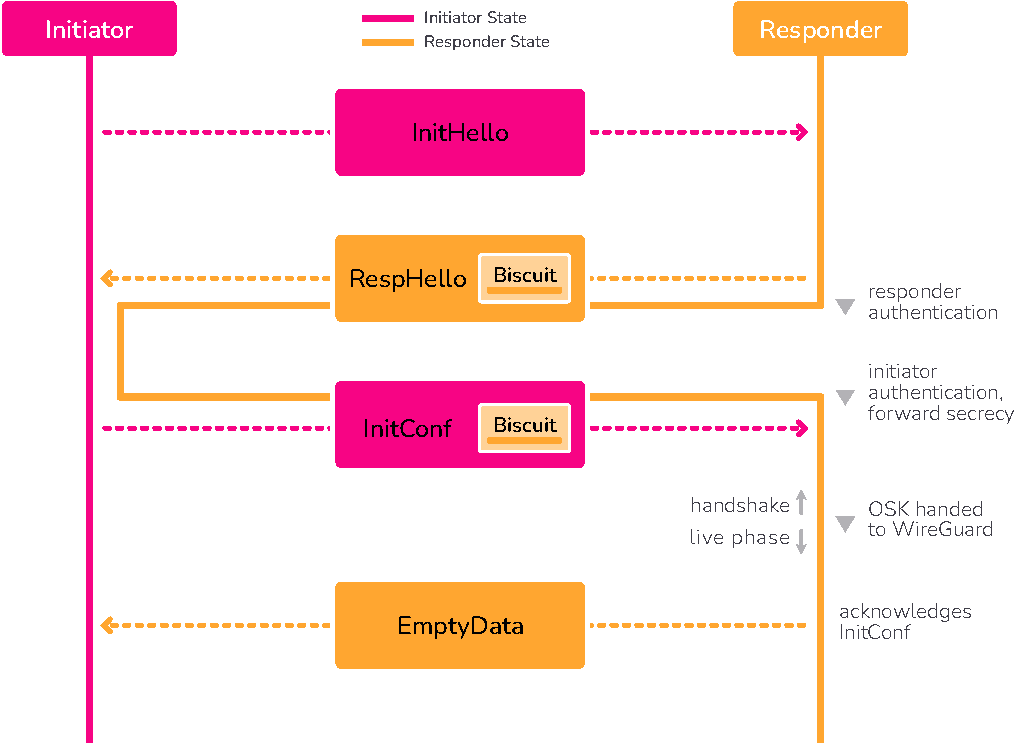
\includegraphics[height=.80\textheight]{graphics/rosenpass-wp-key-exchange-protocol-rgb.pdf}
\end{frame}

\begin{frame}{In Rosenpasss specifically}
  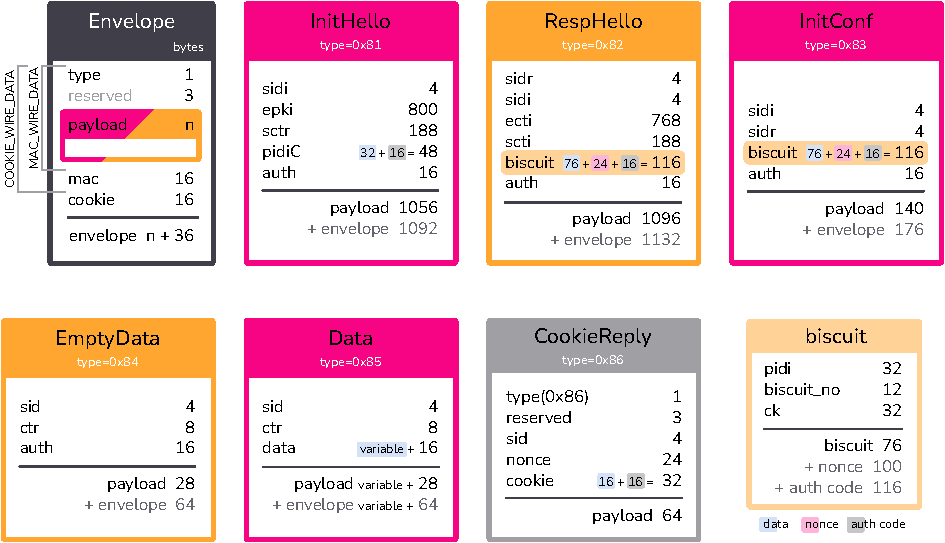
\includegraphics[height=.80\textheight]{graphics/rosenpass-wp-message-types-rgb.pdf}
\end{frame}

\begin{frame}{State Disruption Attacks}
\begin{itemize}
  \item Use the fact that the initiator is not authenticated until their last message
  \item Send faux initiations, overwriting – and thus erasing – the responder's handshake state
  \item Erasing the state aborts protocol execution
  \item PQWG argues: The first package is authenticated using the PSK, therefor sending faux initiations works
  \item Attacker could replay a legitimate message, but…
\end{itemize}
\end{frame}

\begin{frame}{State Disruption Attacks on authenticated initial package}
\begin{itemize}
  \item In Classic WireGuard the initial message (InitHello) is authenticated through static-static Diffie-Hellman
  \item Replay protection uses monotonic counter
  \item WireGuard stores the time of the last initiator $t_i$
  \item When WireGuard receives legitimate initiaton with timestamp $t$, it stores that time $t_i \leftarrow t$a
  \item All InitHello messages with a stale timestamp ($t \le t_i$) get rejected
\end{itemize}
\end{frame}

\begin{frame}{CVE-2021-46873 – Attacking WireGuard through NTP}
\begin{itemize}
  \item The replay protection in classic WireGuard assumes a monotonic counter
  \item But the system time is attacker controlled because NTP is insecure
  \item This generates a kill packet that can be used to render WireGuard keys useless
  \item Attack is possible in the real world!
\end{itemize}
\end{frame}

\begin{frame}{State disruption in Post-Quantum WireGuard}
\begin{itemize}
  \item This mechanism needs an authenticated InitHello message
  \item Post-Quantum WireGuard relies on the $\texttt{psk}$ to provide InitHello authentication
  \item PQWG sets $\texttt{psk} = H(\texttt{spki} \oplus \texttt{spkr})$ to achieve a secret psk.a
  \item Relying on private public keys is absurd
  \item[$\Rightarrow$] With InitHello effectively unauthenticated, attacker can just generate their own kill packet
\end{itemize}
  Solution: Store the responder state in a biscuit (cookie), so there is no state to override.
\end{frame}

\begin{frame}{Biscuits in the protocol flow}
  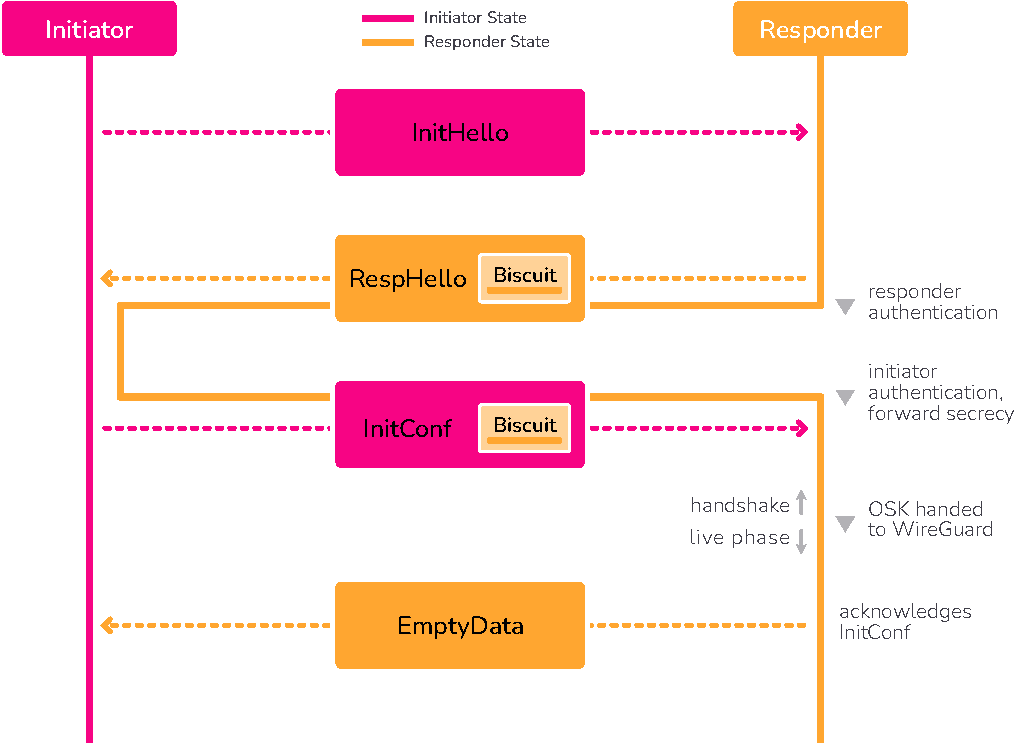
\includegraphics[height=.80\textheight]{graphics/rosenpass-wp-key-exchange-protocol-rgb.pdf}
\end{frame}

\begin{frame}{Biscuits in the messages}
  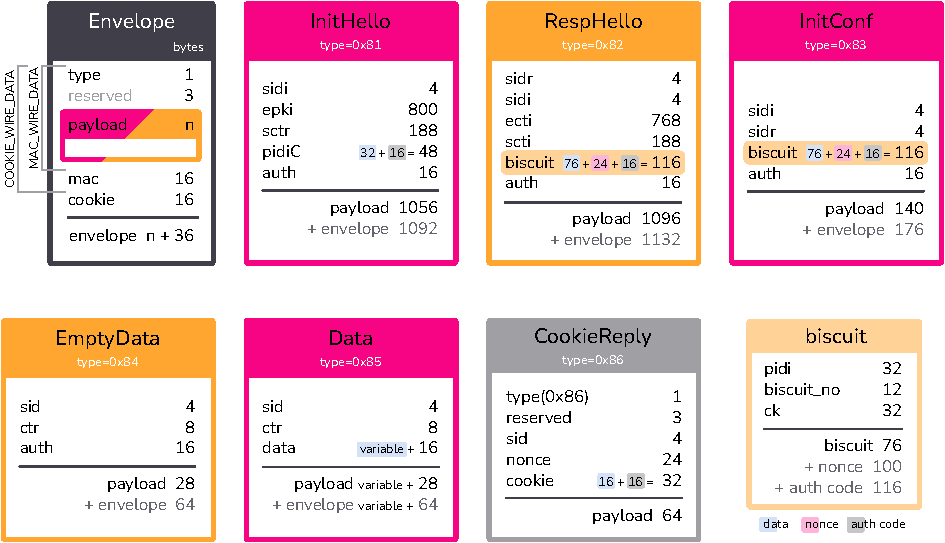
\includegraphics[height=.80\textheight]{graphics/rosenpass-wp-message-types-rgb.pdf}
\end{frame}

\begin{frame}{Biscuits}
  \begin{itemize}
    \item Assumptions such as a monotonic counter are perilous in the real world
    \item Giving the adversary access to state is dangerous
    \item In noise protocols the handshake state is very small (32-64 bytes)
    \item Sending the state to the protocol peer is a viable course of action!
    \item Formalization of State Disruption Attacks covers many attacks of this style
  \end{itemize}
\end{frame}

\begin{frame}{Security proof of rosenpass}
  \begin{itemize}
    \item CryptoVerif in progress (Benjamin Lipp)
    \item Really fast symbolic analysis using ProVerif
  \end{itemize}
\end{frame}

\begin{frame}{Deployment}
  \begin{itemize}
    \item Rust implementation in userspace
    \item Integrates with WireGuard through the PSK feature to provide Hybrid security
  \end{itemize}
\end{frame}

\begin{frame}{Final statements}
  \begin{itemize}
    \item Post-quantum crypto can be deployed now
    \item There are real complexities in protocol design
    \item DoS-Resistance needs formalization work
    \item Availability needs love and attention from cryptographers
    \item Try it out! https://rosenpass.eu/
  \end{itemize}
\end{frame}

%* Problem introduction
%    * Post-quantum-secure authenticated key exchange
%    * Interactive key exchange
%    * No DH
%    * But with KEMs
%        * KEM is non interactive
%        * Gives you secrecy
%        * One-sided auth
%* PQWG
%    * Doing one key encapsulation in both directions
%    * Adding an ephemeral one for forward secrecy
%* State interruption attack
%    * Assumption of monotonic counter is not realistic/broken/…
%    * static keys become essentially useless
%    * Leads to state disruption
%    * Case: WG ohne replay protection (motivation for monotonic counter)
%    * Case: WG mit replay protection
%* Biscuits
%    * No state
%    * Provably avoids state disruption
%    * State machine WG/PQWG: ini
%* 


\end{document}
